\section*{Raccolta dati}
La raccolta dati è basata su due fonti principali: YouTube e [fonte/i covid-19].
\subsection*{Youtube API}
I video in tendenza su youtube variano ogni 15 minuti circa (fonte: \url{https://support.google.com/youtube/answer/7239739?hl=it}) anche se non per forza e solitamente vi è solo una manciata di video che entra/esce dalle tendenze. Per la raccolta di questi dati ci siamo basati sulle funzioni API messe a disposizione da youtube per poter raccogliere i video in tendenza in un dato momento. Le chiavi di richiesta gratuite fornite da Google developer però ci permettono di effettuare una quantità limitata di richieste. 
\\
Abbiamo effettuato sostanzialmente due differenti \textbf{sessioni} di scraping, con metodi leggermente differenti, dovuti allo scopo che ci eravamo prefissati: 
\begin{enumerate}
	\item dal 23 dicembre 2019 al 5 gennaio 2020 (raccolta ogni 30 minuti)
	\item dal 18 marzo 2020 al 6 maggio 2020 (raccolta ogni 6 ore)
\end{enumerate}
Abbiamo deciso di raccogliere dati delle tendenze dei seguenti paesi:

Italia, USA, Regno Unito, India, Germania, Canada, Francia, Corea del sud, Russia, Giappone, Brasile, Messico\\

\subsection*{Prima sessione}
Inizialmente pensavamo di utilizzare i dati per analizzare come, in generale, un video riesce ad arrivare nelle tendenze di youtube e in base a questo fatto analizzare il suo comportamento per quanto riguarda visualizzazioni, likes, dislikes, ecc. La raccolta in questa sessione viene effettuata con lo script \textit{scraper\_timed.py} che sostanzialmente esegue questi passaggi:\\
\\
\begin{algorithm}[H]
	\KwData{country - insieme dei paesi prescelti; videos - insieme di video scaricati da un determinato paese}
	\nl \For{every 30 minutes} {
	\nl \ForEach{country}
	{
		\nl videos = APIrequest(max(50 video), country)\\
		\nl \While {video in tendenza non finiti}
		{
			\nl videos += APIrequest(max(50 video), country) \\
		}
		\nl videos\_fix = arrangeData(videos)\\ 
		\nl saveToCsv(videos\_fix) \\
		\nl videos = $\emptyset$
	}
	}
	\caption{Scraping youtube $\rightarrow$ csv}
\end{algorithm}

%Alternativa per scrivere l'algoritmo
%\begin{enumerate}
%	\item Per ogni paese prescelto
%	\item API request sulle tendenze del momento $\rightarrow$ download di page da 50 video [formato json]
%	\item ripeti 2. finchè scarica tutti i video
%	\item copio le informazioni formattate in formato csv (vedi dopo) 
%	\item ripeti da 2. per ogni paese
%	\item attendi 30 minuti (scheduler)
%	\item ripeti da 1.
%\end{enumerate}
\underline{Nota}: per ogni API request al massimo possiamo scaricare 50 video e ogni paese a un numero diverso di video in tendenza (solitamente 150-200).

In questa sessione abbiamo pensato di salvare i dati in formato \textit{csv}
modo tale che siano facilmente manipolabili. Segue lo schema logico con cui li abbiamo immagazzinati:
\begin{table}[H]
	\centering
	\begin{tabular}{l|l}
		\textbf{Attributo} & \textbf{Descrizione} \\
		\hline
		\textbf{timestamp} & data, ora e minuto della nostra rilevazione \\\hline
		\textbf{video\_id} & identificativo unico del video\\\hline
		\textbf{title} & nome del video per esteso\\\hline
		\textbf{publishedAt} & data di pubblicazione\\\hline
		\textbf{channelId} & identificativo unico del canale che ha pubblicato il video\\\hline
		\textbf{channelTitle} & nome del canale per esteso\\\hline
		\textbf{categoryId} & identificativo unico della categoria\\\hline
		\textbf{trending\_date} & data in cui il video è in tendenza\\\hline
		\textbf{tags} & stringa dei tag usati separati dal carattere "|"\\\hline
		\textbf{view\_count} & numero di visualizzazioni\\\hline
		\textbf{likes} & numero di like (mi piace)\\\hline
		\textbf{dislikes} & numero di dislike (non mi piace)\\\hline
		\textbf{comment\_count} & numero di commenti sotto il video\\\hline
		\textbf{thumbnail\_link} & url all'immagine di copertina del video\\\hline
		\textbf{comments\_disabled} & booleano che dichiara se i commenti sono disabilitati\\\hline
		\textbf{ratings\_disabled} & booleano che dichiara se i like/dislike sono disabilitati\\\hline
		\textbf{description} & descrizione del video\\
		\hline
	\end{tabular}
	\caption{schema degli attributi dei dati csv}
\end{table}

I dati così raccolti sono salvati nella cartella [INSERIRE NOME CARTELLA]

\subsection*{Seconda sessione}

Per la seconda sessione di raccolta, in cui abbiamo deciso di concentrarci sugli effetti che l'epidemia del nuovo virus Covid-19, abbiamo adottato un approccio diverso. Innanzitutto abbiamo deciso di immagazzinare i dati in un database mongoDB nativamente. Pertanto oltre a costruire una pipeline di raccolta che salva i dati direttamente su mongoDB abbiamo deciso parallelamente di immagazzinarli in formato \textit{json}. 

Seconda considerazione è stata data la bassa variabilità dei video raccogliendo i dati ogni 30 minuti, vista nella precedente sessione, abbiamo deciso di effettuare lo scraping ogni 6 ore, in modo da avere 4 rilevazioni durante una giornata. 

A scopo didattico abbiamo inoltre deciso di implementare una piccola pipeline Kafka in cui dividiamo la fase di raccolta dati (\textit{scraper\_producer.py}) e la fase di immagazzinamento (\textit{scraper\_consumer.py}). 

\begin{figure}[H]
	\centering
	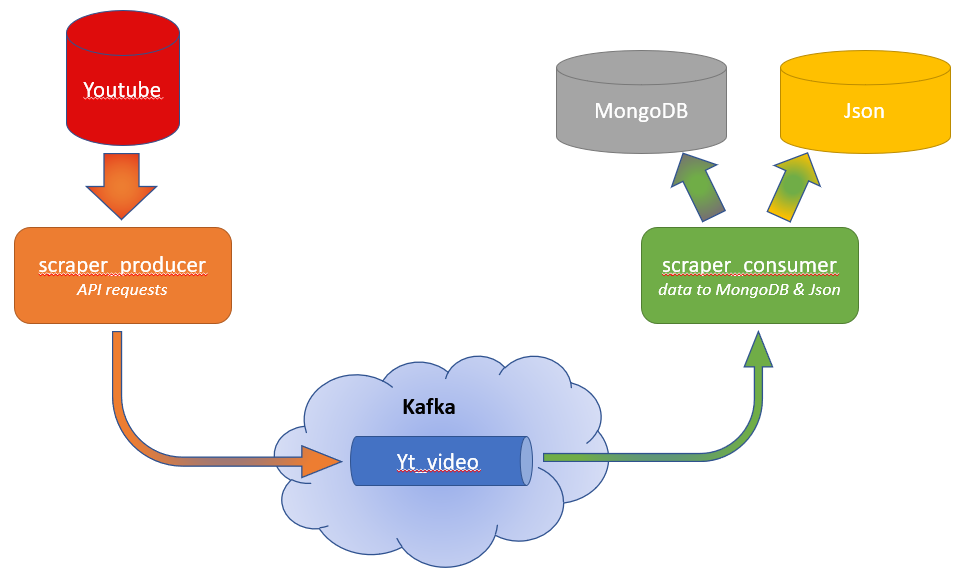
\includegraphics[width=0.8\linewidth]{pics/pipeline.png}
	\caption{pipeline di raccolta dati - seconda sessione}
\end{figure}

Di seguito il dettaglio della computazione dei 2 script:

\begin{algorithm}[H]
	\KwData{country - insieme dei paesi prescelti; videos - insieme di video scaricati da un determinato paese; KafkaProducer(data, channel) - sends data to channel kafka}
	\nl \For{every 6 hours} {
		\nl \ForEach{country}
		{
			\nl videos = APIrequest(max(50 video), country)\\
			\nl KafkaProducer(videos, yt\_video) \\ 
			\nl \While {video in tendenza non finiti}
			{
				\nl videos = APIrequest(max(50 video), country) \\
				\nl KafkaProducer(videos, yt\_video) \\
			}
		}
	}
	\caption{scraper producer}
\end{algorithm}

\begin{algorithm}[H]
	\KwData{KafkaConsumer(channel) - receives data from channel kafka}
	\nl \While{loop} {
		\nl \If{KafkaConsumer(yt\_video) $\ne \emptyset$}
		{
			\nl videos = KafkaConsumer(yt\_video)\\
			\nl videos\_fix = arrangeData(videos)\\ 
			\nl saveToJson(videos\_fix)\\
			\nl saveToMongoDB(videos\_fix)
		}
	}
	\caption{scraper consumer}
\end{algorithm}
I dati così raccolti sono stati salvati in formato json nella cartella [INSERIRE NOME CARTELLA].

\underline{Nota}: abbiamo scelto di salvare i dati in formato Json in modo che fosse facile caricarli in un nuovo server mongoDB e renderli più trasportabili. Per il caricamento vedi lo script: \textit{json\_to\_mongo.py}

Lo schema logico dei documenti json è sostanzialmente lo stesso di quello dei csv visto precedentemente in \textit{Tabella 1} ma con due variazioni:
\begin{itemize}
	\item \textbf{tags} immagazzinati come array di stringhe
	
	Ad esempio:
	
	tags: ["covid-19", "quarantena"]
	\item informazioni relative ai likes, dislikes, view\_count e comment\_count innestati in un oggetto \textbf{statistics}
	
	Ad esempio:
	
	statistics: \{view\_count: 14235,
				likes: 513,
				dislikes: 34,
				comment\_count: 254
				\}
\end{itemize}
\subsection*{Dati Covid-19}

I dati relativi ai Covid-19 sono stati estrapolati da  \href{https://ourworldindata.org/coronavirus-testing}{questo link.} I dati vengono estrapolati in formato \textit{csv}; dopo averli puliti essi contengono le seguenti informazioni:
\begin{table}[H]
	\centering
	\begin{tabular}{l|l}
		\textbf{Attributo} & \textbf{Descrizione} \\
		\hline
		\textbf{iso\_code} & codice unico riferito al paese \\\hline
		\textbf{location} & nome esteso del paese\\\hline
		\textbf{date} & data della rilevazione\\\hline
		\textbf{total\_cases} & numero totale dei casi\\\hline
		\textbf{new\_cases} & nuovi casi registrati in quella giornata.\\\hline

	\end{tabular}
	\caption{Schema degli attributi dei dati sul Covid-19.}
\end{table}

